%We focus now on the case in which the random environment  $\omega(x)_{x \in \ZZ^d} \in [0, 1]^{\ZZ^d}$ is i.i.d. and given a fixed $p \in (0,1]$ we set $p_n=p$, for every $n$. 

%In this text we focus on the homogeneous case, i.e., for every $n$ we set $p_n=p$ \com{no need to say this if we already from the beginning focus on the constant case},  with $p \in (0,1]$ and the marginals of the random element $\pi$ are independent. 

% \subsection{Main results for the $p$-\Name}\label{LGNCLT}\label{sec: res_p-gerw}
% As mentioned in the Introduction the homogeneous case can be reduced to the \Name{}. Specifically, the $p$-\Name{} with a given $\lambda$ in Condition~\ref{condição2} reduces to a \Name{} with $p\lambda$ in Condition $C^+$ in \cite{menshikov2012general}. As a matter of fact, if we denote by $\widetilde{\FF}_n=\sigma(X_1, \ldots, X_n)$, by integrating 
% $\mathbb{E} [ X_{n+1} - X_n | \mathcal{F}_n] \cdot \ell$ with respect to $\pi(X_1), \ldots, \pi(X_n)$ we obtain $\mathbb{E} [ X_{n+1} - X_n | \widetilde{\FF}_n] \cdot \ell\geq p\lambda$, which is Condition $C^+$ in \cite{menshikov2012general} with a $\lambda'=p\lambda$. 
% %
% Despite the close connection with \Name{}, some of the techniques developed to prove results for the  $p$-\Name{} will be useful for the time dependent case. 


% Our first result  is that for every $p \in (0,1]$, the $p$-\Name{} is ballistic in $\ell$ direction. 

% \medskip

% \begin{theorem}[Ballisticity of $p$-\Name{}]\label{teo11}
% Let $X$ be a $p$-\Name{} in direction $\ell \in \mathbb{S}^{d-1}$. %(i.e., satisfies Conditions~\ref{condição1},\ref{condição2} and \ref{condição3}). 
% Then
% \begin{equation*}
% \liminf_{n \to \infty} \frac{X_n \cdot \ell}{n} > 0\;, \quad \text{a.s..}    
% \end{equation*}
% \end{theorem}


% \medskip

% % We could prove that the $p$-\Name{} is transient for any $p > 0$ and find a good lower bound for the probability of the process never return to the initial position. Besides, we are able to see how this bound behaves according to the choice of $p$. 
% %To obtain the ballisticity result we  first upper bound the probability that  the $p$-\Name{} visits less than $n^{1/2+\alpha}$ distinct sites until time $n$ for all $\alpha \in (0, 1/4)$ (see, Proposition~\ref{prop41}) and then, using the latter, we show that the $p$-\Name{} moves ballistically in direction $\ell$ (see, Proposition~\ref{prop42}). The proof is similar to the proof in~\cite{menshikov2012general}. The main difference is that  in~\cite{menshikov2012general}  the set of sites with cookies is deterministic, indeed every site has a cookie, whereas in  our model the set of sites with cookies is random and must be properly controlled. \comu{Acho que podemos remover este parágrafo e fazer a observação antes da prova da Proposição 3. Lembrando que \cite{menshikov2012general} já foi mencionado como a principal referência.}

% \medskip 

% The next two results are the Law of Large Numbers and the Central Limit Theorem which hold for a special case of  $p$-\Name{}. Specifically,   we  need to introduce a fourth condition (see, Condition~\ref{t_k+1 - t_k ind} in Section~\ref{renewalstruc}) which is related to the distribution of the increments of the regeneration times associated to  the $p$-\Name{}. A $p$-\Name{} satisfying this fourth condition will be called \textit{p-Strong General Excited Random Walk} ($p$-\Names).  
% %
% It can be shown (see, Corollary~\ref{pERWcond4})  that the $p$-\Nametwo{} introduced in the  Example in Section~\ref{sec:model} is an example of  $p$-\Names{}. 

% \medskip

% \begin{theorem}[Law of Large Numbers]\label{LLN}
% Assume the process $X$ is a $p$-\Names{} in direction $\ell$ (i.e., satisfies Conditions~\ref{condição1},\ref{condição2}, \ref{condição3} and \ref{t_k+1 - t_k ind}), then there exists  $v \in \mathbb{R}^d$ such that $v \cdot \ell > 0$ and
% \begin{equation}
% \label{Xn/n->v}
% \lim_{n \to \infty} \frac{X_n}{n} = v\;, \quad \text{a.s..}    
% \end{equation}
% \end{theorem}

% \medskip

% Let $X$ be a $p$-\Names{} in direction $\ell$ and $v \in \mathbb{R}^d$   from~\eqref{Xn/n->v}.
% Let us define the process
% \begin{equation}\label{B}
% B_t^n = \frac{X_{\lfloor nt \rfloor} - \lfloor nt \rfloor v}{n^{1/2}}\;,  \ t \ge 0\;.     
% \end{equation}
% %Then, regarding $B_{\cdot}^n$ the following theorem holds. 

% \smallskip

% \begin{theorem}[Central Limit Theorem]\label{CLT} The process $B_{\cdot}^n$ converges in distribution, as $n \to \infty$, to a $d$-dimensional Brownian Motion with a non-degenerate covariance matrix.
% \end{theorem}


\subsection{Main results}\label{main_pn}

Let us recall that we shall focus on the case in which the sequence $\{p_n\}_{n \ge 1}$ is of the form $p_n =\mathcal{C} n^{-\beta} \wedge 1$ for some $\mathcal{C} > 0$. Before we state the main results, let us introduce some notation. Define
\begin{equation}\label{eq:B}
\Hat{B}_t^n := \frac{X_{\lfloor nt \rfloor}}{n^{1/2}} + (nt - \lfloor nt \rfloor)\frac{(X_{\lfloor nt \rfloor + 1} - X_{\lfloor nt \rfloor})}{n^{1/2}} \,, \ t\ge 0 \,,
\end{equation}
where the process $X$ will make reference to a specified process in each Theorem ($p_n$-\Name, $p_n$-\Name*{} or $p_n$-\Nametwo{}). 

Let $C_{\Rs^d}[0,T]$ be the space of continuous functions from $[0,T]$ to $\mathbb{R}^d$ for every $T > 0$. We consider $C_{\Rs^d}[0,T]$ endowed with the uniform topology. Denote by $C_{\Rs^d}[0, \infty)$  the space of continuous functions from $[0,\infty)$ to $\mathbb{R}^d$  endowed  with the metric
\begin{equation}\label{def:rho}
 \rho(f, g) := \sum_{k=1}^{\infty}\frac{1}{2^k} \sup_{0 \le t \le k}(||f(t) - g(t)|| \wedge 1) \,,  \ f, \, g \in  C_{\Rs^d}[0, \infty) \,.
\end{equation}
% It is well-known that if a sequence of random functions in $C_{\Rs^d}[0, \infty)$ converges in probability under the uniform metric in $C_{\Rs^d}[0, T]$ for all $T >0$, then it also converges in probability under the metric $\rho$ \com{this last paragraph  could be removed once we fix the remark 3.1}.

Our first result is a Central Limit Theorem for the $p_n$-\Name* when  $\beta>1/2$ and $d\geq 2$. Before we state our result, for a column vector $a \in \mathbb{R}^d$, let us denote $a^T$ as its transpose.
%Here we will set $p_n = K'n^{-1/2}$ \com{$p_n = K'n^{-\beta}$?} where $\beta > 1/2$ and $K'$ is a positive constant such that $K' \in (0,1]$.


\begin{theorem}\label{pn-WGERW-Gauss}
Let $X$ be a $p_n$-\Name* in direction $\ell$, on $\ZZ^d$, with $d \ge 2$,  $p_n= \mathcal{C}n^{-\beta} \wedge 1$, with $\beta > 1/2$. 
%We define
%\begin{equation*}
    %B_t^{n} = \frac{X_{\lfloor nt \rfloor}}{n^{1/2}} \quad \text{for } t \in \mathbb{R}^{+}\;.
%\end{equation*}
Suppose that 
    \begin{equation*}
    \lim_{k \to \infty} k^{-1/2} \EE\Big[ \sup_{1 \leq i \leq k} \| \xi_i \| \Big]  = 0 \,, \quad \text{ and}
    \end{equation*}
\begin{equation}\label{condGaussiano}
    \frac{1}{n}\sum_{i=1}^{\lfloor nt \rfloor} \xi_i \xi_i^T \xrightarrow[n \to \infty]{} C(t)  \ \textrm{ in probability,}
    \end{equation}
where $C=((c_{i,j}))$ is a continuous $d \times d$ matrix-valued function on $[0,\infty)$ satisfying $C(0) = 0$  and 
\begin{equation*}
\sum_{i,j = 1}^d (c_{i,j}(t) - c_{i,j}(s))\alpha_i \alpha_j \geq 0 \quad \text{for any } \alpha \in \mathbb{R}^d, \quad t > s \geq 0\,.
\end{equation*}
Then $\{\Hat{B}_{\cdot}^n\}_{n\geq 1}$ converges in distribution to a process with independent Gaussian increments with sample paths in $C_{\mathbb{R}^d}[0, \infty)$.
\end{theorem}

\begin{remark}
Let us point out that the $p_n$-\Name* when $\beta>1$ eventually behaves as a $d$-dimensional martingale and in this  case our theorem (essentially) reduces to  \cite[Theorem 7.1.4]{ethier2009markov}.
\end{remark}

% \begin{remark}\label{rem_cond_antes}
% Let us point out that Theorem~\ref{pn-WGERW-Gauss} holds true under slightly weaker conditions. Specifically the Condition~\ref{condiçao I*} and the sequence $\{p_n\}_{n \ge 1}$ can be more general. As it emerges from the proof,  for the statement of Theorem~\ref{pn-WGERW-Gauss} be true we only need that $\sum_{i=1}^{\lfloor nt \rfloor} p_i \EE[||\gamma_i||] = o(\sqrt{n})$ (for more details, see Remark~\ref{rem_cond_frac} ). 
% %
% % \cm{then it will be possible to prove that the second sum portion in~\eqref{p_n-WGERW_incrementos} goes to zero in probability. Hence we finish the poof with Slutsky's Theorem (Theorem 11.4 from~\cite{gut2005probability})}.
% \end{remark}

%\comu{Podemos colocar um remark. Bastaria ter $p_n \sim o(\sqrt{n})$ e $\sup \sqrt{n}p_n E[\|\gamma_n\|] < \infty$} \cm{Coloquei um remark após a prova, naõ exatamente isso.}

%\com{Eu sugiro colocar o remark aqui!}

From Theorem~\ref{pn-WGERW-Gauss} we obtain the following corollary.

\begin{corollary}\label{pnESRW->BM}
Let $X$ be a $p_n$-\Nametwo{} in direction $\ell$ on $\ZZ^d$, with $d \ge 2$, $p_n= Cn^{-\beta} \wedge 1$, with $\beta > 1/2$. %We define
%\begin{equation*}
 %   B_t^{n} = \frac{X_{\lfloor nt \rfloor}}{n^{1/2}} \quad \text{for } t \in \mathbb{R}^{+}\;.
%\end{equation*}
Then $\{\Hat{B}_{\cdot}^n\}_{n\geq 1}$ converges in distribution to a $d$-dimensional Brownian Motion in $C_{\Rs^d}[0,\infty)$.
\end{corollary}

We now consider $\beta = 1/2$. In this case, our results depend on the dimension of the $p_n$-\Nametwo{}. First, we  present a Central Limit Theorem in $d=2$. 

\begin{theorem}\label{pn-ERW-d=2} 
Let $X$ be a $p_n$-\Nametwo{} in direction $\ell$, on $\ZZ^d$ with $d=2$, $p_n= \mathcal{C} n^{-1/2} \wedge 1$. %We define,
%\begin{equation*}
 %   B_t^{n} = \frac{X_{\lfloor nt \rfloor}}{n^{1/2}} \quad \text{for } t \in \mathbb{R}^{+}\;.
%\end{equation*}
Then $\{\Hat{B}_{\cdot}^n\}_{n\geq 1}$ converges in distribution to a $2$-dimensional Brownian Motion in $C_{\Rs^2}[0, \infty)$.
\end{theorem}

\begin{remark}
Note that in Corollary~\ref{pnESRW->BM} and Theorem~\ref{pn-ERW-d=2} the $p_n$-\Nametwo{} under a suitable rescaling converges in distribution to a Brownian Motion and has no ballisticity, differently from what happens in the \Nametwo{} (see~\cite{benjamini2003excited}, \cite{kozma2003excited} and \cite{kozma2005excited}). 
\end{remark}

We now state  our result for the $p_n$-\Nametwo{} in higher dimensions. Here we obtain that the $p_n$-\Nametwo{} suitably rescaled  is tight and every limit point is stochastically dominated in the drift direction $\ell$ from above and below by a Brownian Motion plus a continuous function in $[0, \infty)$. 

Let us define the set $\bD \subset \{e_1, \dots, e_d\}$, where $d \ge 4$ and $1 \leq k:= |\bD| \leq d-3$. Now set $\ell_{\bD}$ as a direction in the unit sphere in dimension $d$, that is, $\ell_{\bD} \in \mathbb{S}^{d-1}$, such that $\ell_{\bD} = \sum_{i=1}^k \alpha_i x_i$, where $\alpha_i \in [0,1]$ and $x_i \in \bD$, both for all $1 \leq i \leq k$. In essence,  $\ell_{\bD}$ is a direction in the unit sphere in dimension $d$ determined by the canonical directions of the set $\bD$. 

We also set $\pi_d$ as the probability that the random walk with increments $\{\xi_i\}_{i\geq 0}$ (i.i.d. with  zero mean and finite variance), never returns to the origin. Moreover if  $X$ be a $p_n$-\Nametwo{} in direction $\ell_{\bD}$ and  $\mathcal{P}_{\bD^c}$ denotes the projection on $\bD^c$, then $\pi_{d-k}$ denotes the probability that the $(d-k)$-dimensional lazy random walk with increments $\{\mathcal{P}_{\bD^c}(\xi_i)\}_{i\geq 0}$  never returns to the origin. Note that $\pi_{d-k} \le \pi_{d}$.

\begin{theorem}\label{pn-ERW-d=>4}
Let $X$ be a $p_n$-\Nametwo{} in direction $\ell_{\bD}$, on $\ZZ^d$ with $d \ge 4$,  $p_n= \mathcal{C} n^{-1/2} \wedge 1$. Then $\{\Hat{B}_{\cdot}^n\}_{n\ge 1}$ is tight in $C_{\Rs^d}[0, \infty)$ and there exist a Brownian Motion $W_{\cdot}$ such that for every limit point $Y_{\cdot}$ of $\{\Hat{B}_{\cdot}^n\}_{n\ge 1}$ 
\begin{align*}
\left\{W_t \cdot \ell_{\bD} + 2 c_1 \sqrt{t}\right\}_{t\ge 0} \preceq \{Y_t \cdot \ell_{\bD}\}_{t\ge 0} \preceq \left\{W_t \cdot \ell_{\bD} + 2 c_2 \sqrt{t}\right\}_{t\ge 0} \,,   
\end{align*}
where $c_1 = \mu_\gamma ( 1-\sqrt{1 -  \pi_{d-k}} )$, $c_2 =\mu_\gamma \sqrt{\pi_d}$ with $\mu_{\gamma} := \EE[\gamma_i \cdot \ell_{\bD}]$ and $\preceq$ means ``stochastically less or equal to''. 
\end{theorem}

Informally speaking, in Theorem~\ref{pn-ERW-d=>4} we obtain  that every limit point of the $p_n$-\Nametwo{} in direction $\ell_{\bD}$ suitably rescaled will be confined within a sort of ``cone'' region, with high probability (see the dashed region in  Figure~\ref{fig:cone}).


\begin{figure}[h]
    \centering
\tikzset{every picture/.style={line width=0.45pt}} %set default line width to 0.75pt        

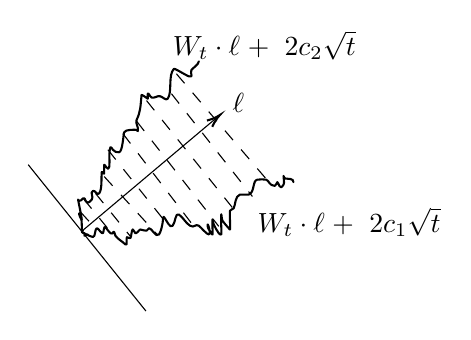
\begin{tikzpicture}[x=0.45pt,y=0.45pt,yscale=-1,xscale=1]
%uncomment if require: \path (0,313); %set diagram left start at 0, and has height of 313

%Straight Lines [id:da8304803087608328] 
\draw    (88,166) -- (182.5,283.5) ;
%Straight Lines [id:da2794399174681552] 
\draw    (131.5,219) -- (240.47,127.29) ;
\draw [shift={(242,126)}, rotate = 139.92] [color={rgb, 255:red, 0; green, 0; blue, 0 }  ][line width=0.75]    (10.93,-3.29) .. controls (6.95,-1.4) and (3.31,-0.3) .. (0,0) .. controls (3.31,0.3) and (6.95,1.4) .. (10.93,3.29)   ;
%Shape: Free Drawing [id:dp08864986808181619] 
\draw  [color={rgb, 255:red, 0; green, 0; blue, 0 }  ,draw opacity=1 ][line width=0.75] [line join = round][line cap = round] (133,221) .. controls (132.67,221) and (132.33,221) .. (132,221) ;
%Shape: Free Drawing [id:dp030738142652891653] 
\draw  [color={rgb, 255:red, 0; green, 0; blue, 0 }  ,draw opacity=1 ][line width=0.75] [line join = round][line cap = round] (131,218) .. controls (131,215.81) and (131.39,207.39) .. (129,205) .. controls (127.73,203.73) and (131,211.8) .. (131,210) .. controls (131,208.74) and (128,194) .. (128,194) .. controls (128,194) and (128.47,194.73) .. (129,195) .. controls (130.07,195.54) and (131.15,193.85) .. (132,193) .. controls (134.46,190.54) and (133.07,201.11) .. (139,194) .. controls (140.93,191.69) and (137.13,188.43) .. (140,187) .. controls (141.7,186.15) and (143.38,191.16) .. (145,189) .. controls (147.51,185.65) and (146.57,175.4) .. (147,172) .. controls (147.18,170.57) and (148.8,174.43) .. (149,173) .. controls (149.33,170.69) and (148.67,168.31) .. (149,166) .. controls (149.11,165.23) and (152.37,171.78) .. (153,168) .. controls (153.7,163.8) and (152.52,155.69) .. (154,152) .. controls (154.35,151.12) and (155.48,153.22) .. (156,154) .. controls (157,155.49) and (159.24,156.35) .. (161,156) .. controls (163.76,155.45) and (164.39,141.83) .. (165,140) .. controls (165.86,137.42) and (174.34,137.91) .. (175,138) .. controls (175.47,138.07) and (175.85,139.45) .. (176,139) .. controls (177.02,135.94) and (173.72,132.56) .. (175,130) .. controls (178.22,123.57) and (178.1,119.01) .. (179,110) .. controls (179.07,109.34) and (183.98,113.09) .. (184,113) .. controls (184.32,111.71) and (183.68,110.29) .. (184,109) .. controls (184.34,107.63) and (185.74,111.37) .. (187,112) .. controls (189.11,113.05) and (191.76,110.25) .. (194,111) .. controls (196,111.67) and (198.74,114.69) .. (200,113) .. controls (203.84,107.88) and (200.1,93.9) .. (205,89) .. controls (205.6,88.4) and (215.1,94.52) .. (217,95) .. controls (221.16,96.04) and (217.77,93.07) .. (219,90) .. controls (219.49,88.77) and (225,85.56) .. (225,83) ;
%Shape: Free Drawing [id:dp1632566533166797] 
\draw  [color={rgb, 255:red, 0; green, 0; blue, 0 }  ,draw opacity=1 ][line width=0.75] [line join = round][line cap = round] (136,222) .. controls (134.95,222) and (134.05,223) .. (133,223) ;
%Shape: Free Drawing [id:dp052118055244864125] 
\draw  [color={rgb, 255:red, 0; green, 0; blue, 0 }  ,draw opacity=1 ][line width=0.75] [line join = round][line cap = round] (132,219) .. controls (131.67,218.67) and (130.85,219.55) .. (131,220) .. controls (131.09,220.28) and (138.31,224) .. (140,224) .. controls (141.99,224) and (141.41,217.8) .. (143,217) .. controls (143.99,216.51) and (147.08,221.92) .. (148,221) .. controls (148.6,220.4) and (148.68,214.95) .. (150,216) .. controls (151.67,217.33) and (152.09,220.05) .. (154,221) .. controls (156.62,222.31) and (155.9,218.9) .. (157,220) .. controls (157.99,220.99) and (157.02,221.62) .. (158,223) .. controls (160.06,225.88) and (163.49,227.49) .. (166,230) .. controls (166.24,230.24) and (166.93,230.33) .. (167,230) .. controls (167.33,228.37) and (166.73,226.64) .. (167,225) .. controls (167.36,222.83) and (168.24,225.88) .. (170,225) .. controls (170.75,224.62) and (171.07,217.38) .. (172,218) .. controls (173,218.67) and (173.15,220.15) .. (174,221) .. controls (174.79,221.79) and (177.08,218.23) .. (178,218) .. controls (179.65,217.59) and (181.48,219.76) .. (183,219) .. controls (183.84,218.58) and (184.09,217.23) .. (185,217) .. controls (186.96,216.51) and (190.55,225.07) .. (193,222) .. controls (194.51,220.11) and (195.71,214.32) .. (196,212) .. controls (196.17,210.64) and (196.14,206.93) .. (197,208) .. controls (199.06,210.58) and (201.85,217.51) .. (204,215) .. controls (206.23,212.39) and (206.14,204.1) .. (209,206) .. controls (212.53,208.35) and (214.34,212.86) .. (218,215) .. controls (221.62,217.11) and (222.14,213.09) .. (225,215) .. controls (226.28,215.85) and (231.94,222.53) .. (233,222) .. controls (234.79,221.11) and (233.25,217.98) .. (233,216) .. controls (232.91,215.26) and (232,213.25) .. (232,214) .. controls (232,218.16) and (233.37,217.73) .. (235,221) .. controls (235.21,221.42) and (235.96,222.47) .. (236,222) .. controls (236.33,218.01) and (235.5,213.97) .. (236,210) .. controls (236.17,208.64) and (236.43,212.75) .. (237,214) .. controls (238.11,216.45) and (239.44,218.81) .. (241,221) .. controls (241.43,221.61) and (242.95,222.74) .. (243,222) .. controls (243.35,216.68) and (242.52,211.31) .. (243,206) .. controls (243.15,204.31) and (243.19,209.51) .. (244,211) .. controls (245.25,213.29) and (247.49,214.88) .. (249,217) .. controls (249.27,217.38) and (249.97,218.47) .. (250,218) .. controls (250.33,213.01) and (249.67,207.99) .. (250,203) .. controls (250.08,201.8) and (252.46,202.07) .. (253,201) .. controls (254.46,198.08) and (254.03,191.19) .. (258,190) .. controls (260.24,189.33) and (262.77,190.67) .. (265,190) .. controls (270.02,188.49) and (267.92,178.51) .. (272,178) .. controls (274.32,177.71) and (276.69,177.67) .. (279,178) .. controls (281.25,178.32) and (281.47,183) .. (286,183) .. controls (286.81,183) and (287.81,180) .. (288,180) .. controls (289.16,180) and (289.79,187.62) .. (293,182) .. controls (294.16,179.97) and (292.62,177.3) .. (293,175) .. controls (293.12,174.26) and (293.27,176.85) .. (294,177) .. controls (296.88,177.58) and (301,176.75) .. (301,180) ;
%Straight Lines [id:da19972782215377438] 
\draw  [dash pattern={on 4.5pt off 4.5pt}]  (130,204) -- (143.5,218.75) ;
%Straight Lines [id:da1175829093412124] 
\draw  [dash pattern={on 4.5pt off 4.5pt}]  (142,189) -- (170,223.5) ;
%Straight Lines [id:da006638707249905007] 
\draw  [dash pattern={on 4.5pt off 4.5pt}]  (149,175.5) -- (192,222.5) ;
%Straight Lines [id:da7126297398825152] 
\draw  [dash pattern={on 4.5pt off 4.5pt}]  (152,154) -- (201,215.5) ;
%Straight Lines [id:da45421712013082516] 
\draw  [dash pattern={on 4.5pt off 4.5pt}]  (164,141) -- (221,215.5) ;
%Straight Lines [id:da09458219023136327] 
\draw  [dash pattern={on 4.5pt off 4.5pt}]  (175,131) -- (241,215.5) ;
%Straight Lines [id:da9986396235508677] 
\draw  [dash pattern={on 4.5pt off 4.5pt}]  (183,114.5) -- (252,200.5) ;
%Straight Lines [id:da8110942219871895] 
\draw  [dash pattern={on 4.5pt off 4.5pt}]  (203,109) -- (268,191.5) ;
%Straight Lines [id:da06174397419817579] 
\draw  [dash pattern={on 4.5pt off 4.5pt}]  (207,93) -- (280,178.5) ;
%Straight Lines [id:da9135651086247871] 
\draw  [dash pattern={on 4.5pt off 4.5pt}]  (132.5,193.5) -- (154,219.75) ;

% Text Node
\draw (250,106.4) node [anchor=north west][inner sep=0.75pt]    {$\ell_{\bD}{}$};
% Text Node
\draw (202,56.4) node [anchor=north west][inner sep=0.75pt]    {$W_{t} \cdot \ell _{\bD}{} +\ 2c_2\sqrt{t}$};
% Text Node
\draw (270,198.4) node [anchor=north west][inner sep=0.75pt]    {$W_{t} \cdot \ell _{\bD}{} +\ 2c_1\sqrt{t}$};

\end{tikzpicture}
\caption{ ``Cone'' region representation around the  direction $\ell_{\bD}$.}
\label{fig:cone}

\end{figure}


Now we propose a conjecture for the $p_n$-\Nametwo{} in direction $\ell \in \mathbb{S}^{d-1}$, on $\ZZ^d$, with $d \ge 3$ and $p_n = \mathcal{C}n^{-1/2} \wedge 1$.

\begin{conjecture}\label{conj_dist}
Let  $X$ be a $p_n$-\Nametwo{} in direction $\ell \in \mathbb{S}^{d-1}$, on $\ZZ^d$ with $d \ge 3$,  $p_n= \mathcal{C} n^{-1/2} \wedge 1$. %We define,
%\begin{equation*}
 %   B_t^{n} = \frac{X_{\lfloor nt \rfloor}}{n^{1/2}} \quad \text{for } t \in \mathbb{R}^{+}\;.
%\end{equation*}
Then  $\{\Hat{B}_{\cdot}^n\}_{n\geq 1}$ converges in distribution to 
$\{W_{t} \cdot \ell + 2 \mu_\gamma \sqrt{\pi_d \, t}\}_{t>0}$,
where $W_{\cdot}$ is a Brownian Motion.
\end{conjecture}

%\cm{The positive constant $c$ in Conjecture~\ref{conj_dist}, we believe that will be such as $c_1 < c < c_2$, where $c_1$ and $c_2$ are from Theorem~\ref{pn-ERW-d=>4}.}

The proof of Theorem~\ref{pn-ERW-d=2} and Theorem~\ref{pn-ERW-d=>4} rely on a control on the range of a $p_n$-\Nametwo{}, which is stated in the following proposition (whose proof is given in Section~\ref{sec:rangeERW}). 

% Considering the representation in \eqref{xn-incremnto1} for $X$ a $p_n$-\Nametwo{} (see, Section~\ref{sec:p_n-ERW}), 
% Let us denote by $\pi_d$ the probability of a random walk with i.i.d. increments (with zero mean and finite variance) given by the corresponding $\{\xi_i\}_{i\geq 0}$ never returning to the origin. 
%
\begin{proposition}\label{prop:RangeERW} 
Let  $X$ be a $p_n$-\Nametwo{} in direction $\ell$, on $\ZZ^d$ with $d\geq 2$, $p_n= \mathcal{C} n^{-1/2} \wedge 1$.
Let $\Rr_n ^X$ be the range of $X$ up to time $n$ (i.e., the number of distinct sites visited by $X$ up to time $n$). Then, for $\delta > \pi_d$
\begin{align*}
    \PP[ \exists n_{\delta} \text{ such that } \forall n \ge n_{\delta} : \ |\Rr_n ^X| \leq \delta n ] = 1 \,.
\end{align*}
\end{proposition}
%
Note that for $d=2$, we have that $\pi_d=0$, whereas for $d\geq 3 $, $\pi_d\in (0,1]$.  Below, we propose a conjecture about the range of the $p_n$-\Nametwo{} on $\ZZ^d$, in direction $\ell \in \mathbb{S}^{d-1}$,  with $p_n= \mathcal{C}n^{-\beta} \wedge 1$, with $\beta\geq 1/2$ and  $d \ge 2$.
%
\begin{conjecture}\label{conj_range}
Let $X$ be a $p_n$-\Nametwo{} in direction $\ell\in \mathbb{S}^{d-1}$, on $\ZZ^d$ with $d\geq 2$, $p_n= \mathcal{C}n^{-\beta} \wedge 1$, with $\beta\geq 1/2$.
Let $\Rr_n ^X$ be the range of the process up to time $n$. Then we have
\begin{equation*}
    \frac{|\Rr_n^X|}{n} \xrightarrow[n \to \infty]{} \pi_d \ \text{ a.s..}
\end{equation*}
\end{conjecture}

\begin{remark}
If  Conjecture~\ref{conj_range} holds true, 
%we could not  prove yet the Conjecture~\ref{conj_dist}. However, 
we would be able to extend the result in Theorem~\ref{pn-ERW-d=>4} to $d=3$ and to any direction in the unit sphere (see Remark~\ref{rem:restriction} in  Section~\ref{sec: d>4}). Specifically, Theorem~\ref{pn-ERW-d=>4} will hold with $c_1 = \mu_\gamma ( 1-\sqrt{1 -  \pi_{d}} )$. Note, however, that this is not yet enough to imply Conjecture~\ref{conj_dist}.
\end{remark}


Table~\ref{table:1} provides a summary of the main results concerning the $p_n$-\Name{}, with $p_n=\mathcal{C}n^{-\beta} \wedge 1$ for different values of $\beta$ and dimension $d$. 

\renewcommand\thetable{\thesection.\arabic{table}}

\begin{table}[!h]    
\caption{Summary of the results for $p_n$-\Name{}.}
\label{table:1}
\begin{tabular}{
|p{0.40\textwidth}
|p{0.54\textwidth}|}
% \hline 
%  $\displaystyle p$-GERW \hfill ($\displaystyle d  \ge 2$, $p\in(0,1]$) &  \ ballisticity in the drift direction for every $\displaystyle p\  >\ 0$. \\
% \hline 
%  $\displaystyle p$-SGERW \hfill ($\displaystyle d  \ge 2$, $p\in(0,1]$) &  \ besides ballisticity, LLN and CLT. \\
% \hline 
%  $\displaystyle p_{n}$-GERW \ \hfill ($\displaystyle \beta <  1/6$, $\displaystyle d \geq 2$) &  \ positive probability of never returning to the origin (in the direction $\ell$) \\
%\hline 
 %$\displaystyle p_{n}$-\Nameone{} \ \ \hfill ($\displaystyle \beta  >1/2$, $\displaystyle d\geq 2$) &  \ convergence in distribution to standard Brownian Motion. \\
\hline 
 $\displaystyle p_{n}$-GERW* \hfill ($\displaystyle \beta   > 1/2$, $\displaystyle d\geq 2$) &   {\it \small Convergence in distribution to a Gaussian Process;} \\
\hline 
 $\displaystyle p_{n}$-\Nametwo{} \hfill ($\displaystyle \beta =1/2$, $\displaystyle d=2$) &  {\it \small Convergence in distribution to a Brownian Motion;} \\
\hline 
 $\displaystyle p_{n}$-ERW \hfill ($\displaystyle \beta =1/2$, $\displaystyle d\geq 4$) &   {\it \small All sub-sequences converge, in distribution,  to a process which is stochastically dominated in the drift direction below and above by a Brownian Motion plus a continuous function.}\\
 \hline
  $\displaystyle p_{n}$-GERW \hfill ($\displaystyle \beta$ small, $\displaystyle d\geq 2$) &   {\it \small Directional transience (see  \cite{alves2022note}).}\\
 \hline
\end{tabular}
\end{table}
%\cm{Hence with the Conjecture~\ref{conj_range} we are able to prove the following result, which is similar with Theorem~\ref{pn-ERW-d=>4}. However we can expand what we obtain for dimension 3 and every direction in the unit sphere.
%\begin{conjecture}\label{conj_dist}
%Let the process $X$ be a $p_n$-\Nametwo{} in direction $\ell \in \mathbb{S}^{d-1}$, in $\ZZ^d$ with $d \ge 3$,  $p_n= C n^{-1/2} \wedge 1$. %We define,
%\begin{equation*}
 %   B_t^{n} = \frac{X_{\lfloor nt \rfloor}}{n^{1/2}} \quad \text{for } t \in \mathbb{R}^{+}\;.
%\end{equation*}
%Then the process $\Hat{B}_{\cdot}^n$ is tight in $C_{\Rs^d}[0, \infty)$ and there exists a Brownian Motion $W_{\cdot}$ such that for every limit point $Y_{\cdot}$ from the process $B_{\cdot}^n$ it holds that
%\begin{align*}
%W_t \cdot \ell + f(t) \preceq Y_t \cdot \ell \preceq W_t \cdot \ell + g(t) \,,   
%\end{align*}
%where $f$ and $g$ are continuous function on $[0, \infty)$, such that $f(t) = c^\prime_1 \sqrt{t}$ and $g(t) = c_2 \sqrt{t}$ with $c_2 > c^\prime_1 >0$. \end{conjecture}}

%\cm{It is important to notice that $c_2$ in Conjecture~\ref{conj_dist} is the same of Theorem~\ref{pn-ERW-d=>4}, however $c^\prime_1 \le c_1$.}



% We now provide our last result, which states that, for $\beta<1/6$ and $d\geq 2$ the $p_n$-\Name{} in direction $\ell$, in $\ZZ^d$ has a positive probability of never returning to the origin in the $\ell$ direction. 
% . Now we set $\beta < \alpha < 1/6$ and $d \ge 2$, where $\alpha$ is establish in Proposition~\ref{prop41}. We will obtain that the $p_n$-\Name{} in direction $\ell$, in $\ZZ^d$ has a positive probability that never returns to the origin in the $\ell$ direction.}



% Before stating the theorem, we  need some notation. 
% for our next result  \cm{which provides a uniform lower bound on the probability of the $p_n$-\Name{} in direction $\ell$ never return to the origin in this direction.} 
% For every $\ell \in \mathbb{S}^{d-1}$, let $\mathbb{M}_{\ell}$ denote the positive half-space in direction $\ell$, that is, $\mathbb{M}_{\ell} = \{ x \in \ZZ^d : x \cdot \ell > 0 \}$. 
% We define $A$ as the \textit{excitation-allowing set}, which means the set of sites where there is the possibility of having cookies (see Condition~\ref{condição2A}). We set the event $\{\eta(X_0) = \infty\}$ as the event in which  the process $X$ never returns to the origin in the drift direction.


% \begin{theorem}\label{prop43_pnn0}
% Let $X$ be a $p_n$-\Name~in direction $\ell$, in $\ZZ^d$ with $d \ge 2$, where  $p_n = (q_0 +n)^{-\beta}$, with $\beta<1/6$,  $q_0$ is a non negative integer and excitation-allowing set $A \subset \mathbb{Z}^d$ such that $\mathbb{M}_{\ell} \subset A$. There exists $\psi > 0$ depending on the parameters of the model  such that
% \begin{equation*}
% \PP\left[ \eta(X_0) = \infty \right] \geq \PP\left[ X_n \cdot \ell > 0 \text{  for all  } n\geq 1\right] \geq \psi\, . 
% \end{equation*}
% % where $\psi = h^{\lceil r^{-1} \rceil C \left(\frac{3}{\lambda} \right)^{\frac{1}{\delta -1}}} c$,  $c \in (0, 1)$, $\delta = (2-\alpha+\beta)(1/2 + \alpha-\beta)$, 
% % \begin{align*}
% % C & = K^{\frac{1}{\delta-1}} \left( \eta + \lceil r^{-1} \rceil^{\frac{1}{\delta-1}}\right) + q_0\;, 
% % \\
% % \eta & = \left( \frac{ 2-\alpha+\beta}{\vartheta_1 \varphi_1}\right)^{\frac{1}{\varphi_1}}  \, , \quad \varphi_1  = \min \left\{ \alpha-\beta, (2-\alpha+\beta)\vartheta_2 \right\}\, , \nonumber
% % \end{align*}
% % and $\vartheta_1$, $\vartheta_2$ are as in Proposition~\ref{prop42_pnn0}. \comu{Fica um pouco estranho esta referência a proposição 3.3, porque ela só aparece no final do texto. Acho melhor definir $\vartheta_1$, $\vartheta_2$ e fazer menção aos valores aqui no enunciado da 3.3 (mesmo sabendo que usamos a 3.3 para provar o teorema.}
% \end{theorem}


% \br{
% \begin{theorem}\label{prop43_pnn0}
% Let $X$ be a $p_n$-\Name~in direction $\ell$ with $p_n = (q_0 +n)^{-\beta}$, where $q_0$ is a non negative integer and excitation-allowing set $A \subset \mathbb{Z}^d$ such that $\mathbb{M}_{\ell} \subset A$. There exists $\psi > 0$ depending on $d$, $K$, $h$, $r$, $\lambda$, $\alpha$ and $\beta$ such that
% \begin{equation*}
% \PP\left[ \eta(X_0) = \infty \right] \geq \PP\left[ X_n \cdot \ell > 0 \text{  for all  } n\geq 1\right] \geq \psi\, ,
% \end{equation*}
% where $\psi = h^{\lceil r^{-1} \rceil C \left(\frac{3}{\lambda} \right)^{\frac{1}{\delta -1}}} c$,  $c \in (0, 1)$, $\delta = (2-\alpha+\beta)(1/2 + \alpha-\beta)$, 
% \begin{align*}
% C & = K^{\frac{1}{\delta-1}} \left( \eta + \lceil r^{-1} \rceil^{\frac{1}{\delta-1}}\right) + q_0\;, 
% \\
% \eta & = \left( \frac{ 2-\alpha+\beta}{\vartheta_1 \varphi_1}\right)^{\frac{1}{\varphi_1}}  \, , \quad \varphi_1  = \min \left\{ \alpha-\beta, (2-\alpha+\beta)\vartheta_2 \right\}\, , \nonumber
% \end{align*}
% and $\vartheta_1$, $\vartheta_2$ are as in Proposition~\ref{prop42_pnn0}. \comu{Fica um pouco estranho esta referência a proposição 3.3, porque ela só aparece no final do texto. Acho melhor definir $\vartheta_1$, $\vartheta_2$ e fazer menção aos valores aqui no enunciado da 3.3 (mesmo sabendo que usamos a 3.3 para provar o teorema.}
% \end{theorem} }



% Figure~\ref{table:1} provides a summary of the main results concerning $p$-\Name{} and the $p_n$-\Name{}, with $p_n=\mathcal{C}n^{-\beta} \wedge 1$ for different values of $\beta$ and dimension $d$.

% \begin{figure}[!h]
%         \centering
        
% \begin{tabular}{|p{0.40\textwidth}|p{0.54\textwidth}|}
% % \hline 
% %  $\displaystyle p$-GERW \hfill ($\displaystyle d  \ge 2$, $p\in(0,1]$) &  \ ballisticity in the drift direction for every $\displaystyle p\  >\ 0$. \\
% % \hline 
% %  $\displaystyle p$-SGERW \hfill ($\displaystyle d  \ge 2$, $p\in(0,1]$) &  \ besides ballisticity, LLN and CLT. \\
% % \hline 
% %  $\displaystyle p_{n}$-GERW \ \hfill ($\displaystyle \beta <  1/6$, $\displaystyle d \geq 2$) &  \ positive probability of never returning to the origin (in the direction $\ell$) \\
% %\hline 
%  %$\displaystyle p_{n}$-\Nameone{} \ \ \hfill ($\displaystyle \beta  >1/2$, $\displaystyle d\geq 2$) &  \ convergence in distribution to standard Brownian Motion. \\
% \hline 
%  $\displaystyle p_{n}$-GERW* \hfill ($\displaystyle \beta   > 1/2$, $\displaystyle d\geq 2$) &  \ convergence in distribution to a Guassian Process \\
% \hline 
%  $\displaystyle p_{n}$-\Nametwo{} \hfill ($\displaystyle \beta =1/2$, $\displaystyle d=2$) &  \ convergence in distribution to a Brownian Motion \\
% \hline 
%  $\displaystyle p_{n}$-ERW \hfill ($\displaystyle \beta =1/2$, $\displaystyle d\geq 4$) &  \ all sub-sequences converge, in distribution,  to a process which is stochastically dominated in the drift direction below and above by a Brownian Motion plus a continuous function.\\
%  \hline
% \end{tabular}
% \caption{Summary of the results for \Name{}.}
% \label{table:1}
% \end{figure}



% \cm{We now present the $p_n$-\Name{}, a special type of the $\lambda_n$-\Name{} as we will see. Set $\{U_i\}_{i \geq 1}$ as a sequence of i.i.d. random variables with uniform distribution in $[0,1]$ and a sequence $\{p_n\}_{n \ge 1}$ such that $p_n \in (0, 1]$ for all $n \ge 1$. For $i\ge 1$ we define $E_i$ as the event that the process $\{X_n\}_{n \geq 0}$ is, at time $i$,  in an already visited site, i.e.,  $E_i:= \{ \exists\;  k < i \; \text{ such that }\;  X_k = X_i \}$ and $E_0:= \emptyset$. We write $\{X_n\}_{n \geq 0}$ as
% \begin{align}\label{xn-incremnto1}
% \begin{split}
% X_n & = \sum_{i=1}^n  (X_i - X_{i-1})
% \\
% & = \sum_{i=1}^n \big(1_{\{E_{i-1}\}} \xi_i + 1_{\{E_{i-1}^c\}} 1_{\{U_{i} > p_{i} \}} \xi_i + 1_{\{E_{i-1}^c\}}1_{\{ U_{i} \leq p_{i}\}} \gamma_i \big) \,. 
% \end{split}
% \end{align}
%where $\{\xi_i, \FF_i\}_{i \geq 1}$ is an increment of a $d$-martingale with zero mean and $\{\gamma_i, \FF_i\}_{i\geq 1}$ is a random vector such that $\EE[\gamma_i \cdot \ell | \FF_{i-1}] \ge \lambda$ for all $i \ge 1$.  
% We also have that $|| \xi_i||<K$ as well as $||\gamma_i||<K$ for all $i \ge 1$. We can explain the model as the following, given the sequence  $\{p_n\}_{n \ge 1}$, if at time $n$ the process visits a site for the first time, it finds a cookie with probability $p_n$ (thus gaining a drift). Otherwise, with probability $1-p_n$, it finds no cookie (no drift) and behaves as a $d$-martingale with zero-mean vector. Otherwise, if the process has already visited the site, there is no cookie and the process acts again as a $d$-martingale with zero-mean vector.}

% \cm{The $p_n$-\Name{} can be reduced to the $\lambda_n$-\Name{}. Specifically, the $p_n$-\Name{} with a given $\lambda$ reduces to a $\lambda_n$-\Name{} with $p_n\lambda$ in Condition~\ref{condição2}. As a matter of fact, if we denote by $\widetilde{\FF}_n=\sigma(X_1, \ldots, X_n)$, by integrating 
% $\mathbb{E} [ X_{n+1} - X_n | \mathcal{F}_n] \cdot \ell$ with respect to $U_1, \ldots, U_n$ we obtain $\mathbb{E} [ X_{n+1} - X_n | \widetilde{\FF}_n] \cdot \ell\geq p_n\lambda$, which is Condition~\ref{condição2} in with a $\lambda_n = p_n\lambda$.}

%\comu{Se vamos fixar $\lambda_n = \lambda (n_0+n)^{-\beta}\,$, $n\ge 0$, faremos aqui.}

%%%%%%%%%%%%%%%%%%%%%%%%%%%%%%%%%%%%%%%%%
%%%%%%%%%%%%%%%%%%%%%%%%%%%%%%%%%%%%%%%%%
%%%%%%%%%%%%%%%%%%%%%%%%%%%%%%%%%%%%%%%%%
%\subsection{Main results for the $\lambda_n$-\Name}\label{main_pn}

%\cm{We provide our main result, which states that, there exists a $\beta > 0$ which the $\lambda_n$-\Name{} in direction $\ell$, in $\ZZ^d$ has a positive probability of never returning to the origin in the $\ell$ direction.} 
% . Now we set $\beta < \alpha < 1/6$ and $d \ge 2$, where $\alpha$ is establish in Proposition~\ref{prop41}. We will obtain that the $p_n$-\Name{} in direction $\ell$, in $\ZZ^d$ has a positive probability that never returns to the origin in the $\ell$ direction.}

% For every $\ell \in \mathbb{S}^{d-1}$, let $\mathbb{M}_{\ell}$ denote the positive half-space in direction $\ell$, that is, $\mathbb{M}_{\ell} = \{ x \in \ZZ^d : x \cdot \ell > 0 \}$.
% Our main result is stated below:

% \begin{theorem}\label{prop43_pnn0}
% Let $X$ be a  $\lambda_n$-\Name{} in direction $\ell$ with excitation set $A \supset \mathbb{M}_{\ell}$.  There exists $\beta_0 < 1/6$ such that if for some $n_0 \in \mathbb{N}$, $\lambda >0$ and $\beta<\beta_0$, we have $\lambda_n \ge \lambda (n_0+n)^{-\beta}$ for every $n\ge 1$, then
% $$
% \PP \big( \lim_{n \rightarrow \infty} X_n \cdot \ell = \infty \big) > 0\,.
% $$
% \end{theorem}

% \begin{remark}\label{rem:sub-balistic}
% 1. If $\lambda_n$ is $O(n^{-\beta})$, then the  $\lambda_n$-\Name{} is not ballistic since the total mean drift accumulated by time $n$ is bounded by  $n^{1-\beta}$. We conjecture that $\lim_{n \rightarrow \infty} X_n \cdot \ell = \infty$ holds almost surely, and even that $\liminf_{n \rightarrow \infty} n^{\beta - 1} X_n \cdot \ell > 0$ almost surely. 2. The condition $\beta < 1/6$ in the statement of Theorem \ref{prop43_pnn0} follows from limitations in our proof. We also conjecture that the result holds for $\beta < 1/2$. For a discussion on the case $\beta \ge 1/2$ see \cite{AIV}.
% \end{remark}

%This text is organized as follows: The renewal structure and the proof of the main results for the $p$-\Name{} are presented in Section \ref{renewalstruc}. Our main contributions are given in Section \ref{resultados_pn}
%and  \ref{proofpropR_n},where we study the $p_n$-\Name{}, with $p_n=n^{-\beta}$. We prove several asymptotic results depending on the value of $\beta$ and on the dimension $d$ (see Section~\ref{prova-pn-WGERW},~\ref{prova-pn-ERW_d=2},~\ref{sec: d>4} and~\ref{sec:d>2_b<1/6}). In Section~\ref{sec:rangeERW} we provide the proof of Proposition~\ref{prop:RangeERW}, in which we analyze the asymptotic behavior of the range of the $p_n$-\Nametwo{} in $d \ge 2$ and $\beta = 1/2$. Finally,  Appendix~\ref{sec:appendixA}, \ref{sec:appendixB} contain some proofs which were omitted in the main text and Appendix~\ref{sec:appendixC} some auxiliary results.

%%%%%%%%%%%%%%%%%%%%%%%%%%%%%%%%%%%%%%%%%
%%%%%%%%%%%%%%%%%%%%%%%%%%%%%%%%%%%%%%%%%
%%%%%%%%%%%%%%%%%%%%%%%%%%%%%%%%%%%%%%%%%


%\subsection{The model}\label{sec:model}
% We now formally introduce the $p_n$-\Name{}. Recall that $d \ge 2$ is the fixed dimension and let $\{p_n\}_{n \ge 1}$ be a sequence of parameters with $p_n \in (0, 1]$ for all $n \ge 1$.
% In a broader sense our process is a random element $(X,\pi)$ of $(\mathbb{Z}^d)^{\mathbb{Z}_+} \times [0, 1]^{\ZZ^d}$ endowed with the product Borel $\sigma$-algebra. The second coordinate $\pi = \{\pi(x)\}_{x \in \ZZ^d} \in [0, 1]^{\ZZ^d}$ is a random element whose marginals have uniform distribution in $[0,1]$ \and independents. We denote by $Q$ the probability law of $\pi$.  
% The first coordinate $X = \{ X_n \}_{n \geq 0}$ is a $\ZZ^d$ valued process with $X_0=0$ which is adapted to a filtration  $\mathcal{F} = \{ \mathcal{F}_n \}_{n \geq 0}$, where $\FF_n = \sigma(X_1,\dots, X_n, \pi(X_1), \dots,$ $\pi(X_n))$ and $\sigma(Y)$ represents the smallest $\sigma$-algebra generated by a random vector $Y$. We denote the law of $(X,\pi)$ by $\PP$ and by $\mathbb{E}$ its expectation, we can think of $\PP$ as the semi-direct measure $Q \otimes P_{\hat \pi}$, where $P_{\hat \pi}$ is the quenched measure for $X$, i.e., the conditional probability law of $X$ given a realization $\hat \pi$ of $\pi$. Now fix $\ell \in \mathbb{S}^{d-1}$, where $\mathbb{S}^{d-1}$ is the unit sphere of $\mathbb{R}^d$, and let $||\cdot||$ be the euclidean norm in $\mathbb{R}^d$. The process $X$ is called a $p_n$-\Name{} in direction $\ell$, if it satisfies the following conditions:

% \begin{condition}[Bounded increments]\label{condição1}
% There exists a constant $K > 0$ such that $ \sup_{n \geq 0} || X_{n+1} - X_{n} || < K$ on every realization. 
% \end{condition}

% \begin{condition}\label{condição2}
%  There exists $\lambda > 0$ such that: 

% \begin{itemize}
%     \item almost surely on the event $\{ X_k \neq X_n \text{ for all } \; k < n \}$, either
% $$
%     \mathbb{E} [ X_{n+1} - X_n | \mathcal{F}_n] \cdot \ell  \geq \lambda\;, \  \text{if $\pi(X_n) \leq p_n$}\, ,
% $$
% or
% $$
%     \mathbb{E} [ X_{n+1} - X_n | \mathcal{F}_n] =0 \;, \ \text{if $\pi(X_n) >p_n$}\, .
% $$
%     \item almost surely on the event $\{ \exists\,  k < n  \text{ such that }  X_k = X_n \}$,
%     \[
%      \mathbb{E} [ X_{n+1} - X_n | \mathcal{F}_n] = 0\, .
%     \]
% \end{itemize}
% \end{condition}


% \begin{condition}\label{condição3}
%  There exist $h, r > 0$ such that

% \begin{itemize}
%     \item {\rm Uniformly elliptic in direction $\ell$:}  for all $n$
% \begin{equation} \label{3 1.4}
% \tag{UE1}\PP \left[ \left( X_{n+1} - X_n \right) \cdot \ell > r | \mathcal{F}_n \right] \geq h\;, \; {a.s..}
% \end{equation}
% \item {\rm Uniformly elliptic on the event $\{\mathbb{E} [ X_{n+1} - X_n | \mathcal{F}_n] = 0\}$:} on the event $ \{ \mathbb{E} [ X_{n+1} - X_n | \mathcal{F}_n] = 0 \}$,  for all $\ell' \in \mathbb{S}^{d-1}$,  with $|| \ell '|| = 1$
% \begin{equation} \label{3 1.5}
% \tag{UE2}\PP \left[ \left( X_{n+1} - X_n \right) \cdot \ell ' > r | \mathcal{F}_n \right] \geq h\;, \; {a.s..}
% \end{equation}
% \end{itemize}
% \end{condition}

% We now present a helpful way to write the $p_n$-\Name{}, especially in the proofs. Let $\{X_n\}_{n \ge 0}$ be a $p_n$-\Name{} in direction $\ell$. Increasing the probability space the following representation for the process holds: Set $\{U_i\}_{i \geq 1}$ as a sequence of i.i.d. random variables with uniform distribution in $[0,1]$~\footnote{Note that this sequence is part of the marginals of  $\pi$. To avoid clutter, we set this i.i.d. uniform distribution as $\{U_i\}_{i \geq 1}$ from now on.}. For $i\ge 1$ we define $E_i$ as the event that the $p_n$-\Name{} is, at time $i$,  in an already visited site, i.e.,  $E_i := \{ \exists\;  k < i \; \text{ such that }\;  X_k = X_i \}$ and $E_0 := \emptyset$. 
% %
% We can write $\{X_n\}_{n \geq 0}$ as

% \begin{align}\label{xn-incremnto1}
% \begin{split}
% X_n & = \sum_{i=1}^n  (X_i - X_{i-1})
% \\
% & = \sum_{i=1}^n \big(1_{\{E_{i-1}\}} \xi_i + 1_{\{E_{i-1}^c\}} 1_{\{U_{i} > p_{i} \}} \xi_i + 1_{\{E_{i-1}^c\}}1_{\{ U_{i} \leq p_{i}\}} \gamma_i \big) \,, 
% \end{split}
% \end{align}
% where $\{\xi_i, \FF_i\}_{i \geq 1}$ is an increment of a $d$-martingale with zero mean and $\{\gamma_i, \FF_i\}_{i\geq 1}$ is a random vector such that $\EE[\gamma_i \cdot \ell | \FF_{i-1}] \ge \lambda$ for all $i \ge 1$.  Note that due to Condition~\ref{condição1} (bounded jumps), we also have that $|| \xi_i||<K$ as well as $||\gamma_i||<K$.
%When we assume the process is a submartingale in the direction $\ell$, we mean
%\begin{itemize}
   % \item $\EE|\gamma_n \cdot \ell| < \infty $ for all $n$. 
%    \item $\gamma_n \cdot \ell$ is adapted to $\FF_n$.
 %   \item $\EE[\gamma_{n+1} \cdot \ell| \FF_n] \geq \gamma_n$.
%\end{itemize}















